

%Zur Dekodierung auf eine bestimmte Lautsprecheranordnung wird eine Matrix aus virtuellen Mikrofonen berechnet, woraus sich eine Tabelle mit Gain-Werten ergibt. Diese Tabelle besteht aus einer Spalte für jeden Lautsprecherkanal und kann die einzelnen Frequenzbins in einem VBAP-Verfahren den enstprechenden Lautsprechern zuordnen. In dieser Seminararbeit wurden dabei zwei Ansätze für die Dekodierung verglichen: Einerseits die direkte Dekodierung auf die physische Lautsprecheranordnung des Wiedergabesystems, und andererseits ein allgemeiner Ansatz womit die Dekodierung auf eine t-Design Lautsprecheranordnung erfolgt. Dieser Dekodierungsansatz hat den Vorteil, dass die Wiedergabeanordnung zum Zeitpunkt des Upmixings nicht vorgegeben sein muss. Auch für die Klangqualität ergeben sich daraus Vorteile, welche im Hörversuch besprochen werden.

Im Frequenzbereich wird die Dekodierungsmatrix von virtuellen Mikrofonen auf jeden Spektralblock angewandt, um die vier Eingangskanäle in eine höhere Kanalzahl zu wandeln.

TODO: WAS SIND VIRTUELLE MIKROFONE?

In dieser Seminararbeit wurden dabei zwei Ansätze für die Dekodierung verglichen: Einerseits die direkte Dekodierung auf die physische Lautsprecheranordnung des Wiedergabesystems, und andererseits ein allgemeiner Ansatz womit die Dekodierung auf eine t-Design Lautsprecheranordnung erfolgt. Dieser Dekodierungsansatz hat den Vorteil, dass die Wiedergabeanordnung zum Zeitpunkt des Upmixings nicht vorgegeben sein muss.

Bei einem 9-Design (Abb. \ref{fig:tdesign_image}) ergibt sich eine sphärische Anordnung von 48 Schallquellen, welche die verlustlose Konvertierung zwischen B-Format und einer solchen Lautsprecheranordnung bietet.

\begin{figure}[!ht]
  \centering
  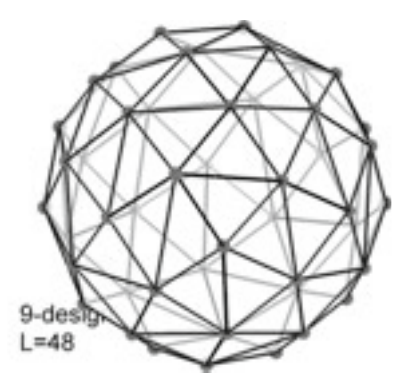
\includegraphics[width=0.35\textwidth]{implementierung/plots/t-design.png}
  \caption{9-Design T-Design \cite{ambi-book}}
  \label{fig:tdesign_image}
\end{figure}

%Zur Dekodierung wird in Octave also eine Matrix mit Lautsprechergewichten für Schalleinfallsrichtungen erstellt. Somit kann einer gegebenen frequenzabhängigen Richtung (bestehend aus Azimuth und Elevation), ein bestimmter Gain-Wert am entsprechenden Lautsprecherkanal zugeordnet werden.
